\documentclass[10pt]{article}
\usepackage[margin=0.72in]{geometry}
\usepackage[T1]{fontenc}
\usepackage{graphicx}
\usepackage{amsmath}
\usepackage{amssymb}
\usepackage{array}
\setlength{\parskip}{0.45em}
\setlength{\parindent}{0pt}
\begin{document}
\begin{center}
{\Large\bfseries Semaev decomposition certificate: Lean decision theorem}\par
{\small 2026-10-21; THM-SEMAEV-FALL1 Lemma 3; TASK-20260916-b55948}
\end{center}

\textbf{Scope.} This theorem checks a proposed finite-field point
decomposition. It does not assert that one exists, estimate its probability,
validate a particular archived run, or bound a solver's cost.

\section*{Predicate and checked theorem}
Let $F$ be finite, $K$ a field with decidable equality and an $F$-algebra
structure, and $V=\operatorname{span}_F\{b_1,\ldots,b_B\}\subseteq K$.
For a tuple of affine Weierstrass points $P_1,\ldots,P_m$, the checker
rejects infinity, checks the curve equation and $x(P_i)\in V$, and compares
the point sum with a supplied target $R$. Lean proves:
\[
 \operatorname{decide}(\operatorname{Valid}(P_1,\ldots,P_m;R))=\texttt{true}
 \quad\Longleftrightarrow\quad
 \bigl(\forall i,\ P_i\text{ is finite},\ E(P_i),\ x(P_i)\in V\bigr)
 \ \land\ \sum_i P_i=R.
\]
The span decision searches the finite coefficient space $F^B$. A separate
raw-coordinate checker rejects pairs failing the explicit curve equation,
reifies valid pairs as Mathlib points, and uses the same group law. Its iff
theorem connects the raw path to curve, span, and sum conditions.

\begin{center}
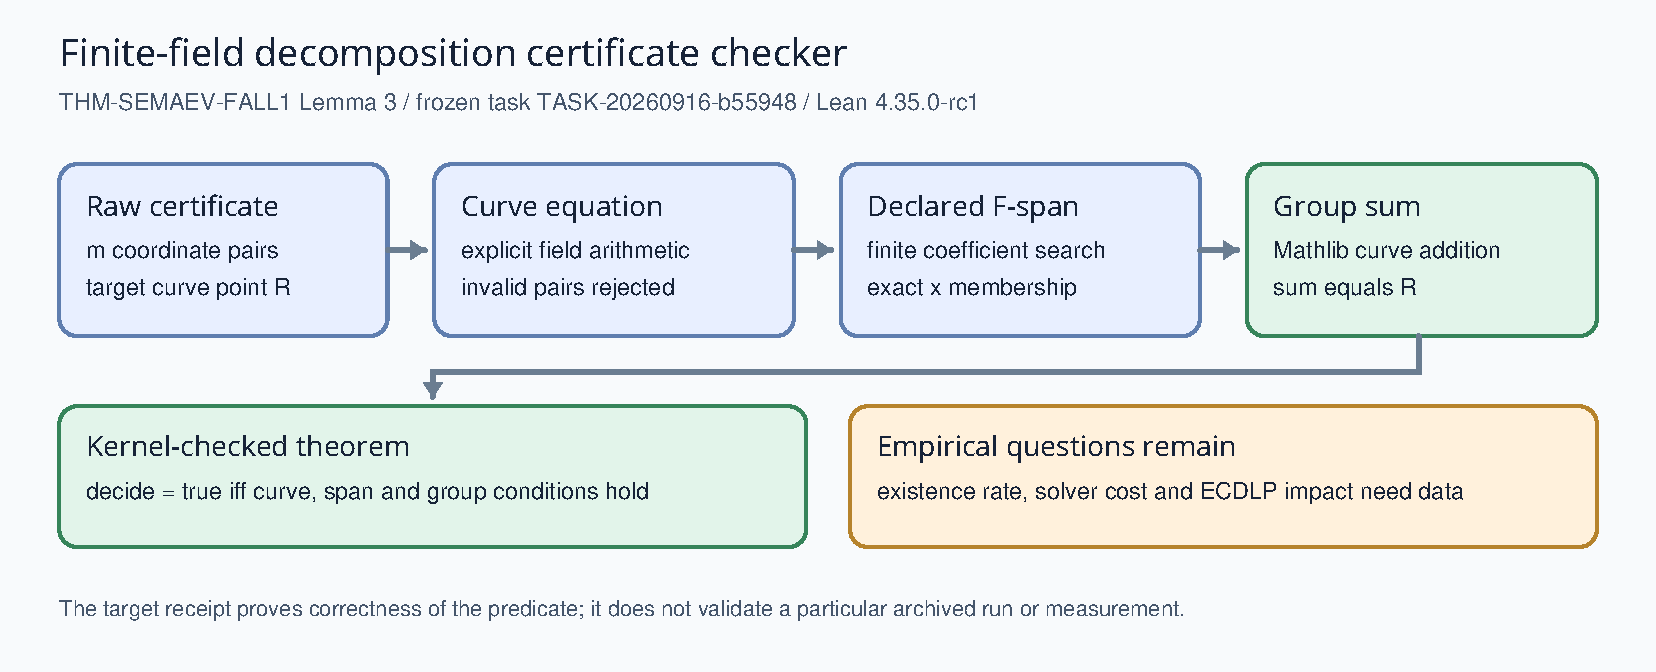
\includegraphics[width=\linewidth]{diagram.pdf}
\end{center}

\section*{Validation and limits}
\begin{tabular}{|p{0.31\linewidth}|p{0.59\linewidth}|}\hline
Check & Observed result \\ \hline
Pinned Lean workspace & Lake build passed 2,075 jobs on Lean 4.35.0-rc1. Project axiom audit passed 494 theorem declarations using standard axioms only. \\ \hline
Frozen certificate target & Machine verified; source commit and task, theorem, toolchain, and manifest hashes bound in the receipt. Independent semantic review remains pending. \\ \hline
Complete target corpus & 64 machine verified; zero failed; zero infrastructure failures; two theorem files absent (NCP reachability and commutator-ideal refutation). \\ \hline
\end{tabular}

The first target attempt failed the verifier's named-theorem audit because
it exported only a \texttt{Decidable} instance. The final source retains
that instance and proves the named \texttt{decide = true} equivalence.
No numerical dashboard or performance graph changed: no new timing datum
was produced. Membership search can be expensive for large $F^B$; this
proof gives no runtime bound or decomposition-rate estimate.

\end{document}
